\section{Laboratorium V}\label{sec:lab5}

\subsection{Wybrany sprzęt}\label{subsec:lab5-hw}

Do tego laboratorium wykorzystano moduł \emph{Traffic pHAT}.
Moduły \emph{pHAT} różnią~się od~\emph{HAT} w~taki~sposób, że~nie~posiadają czipa kontrolnego powiadamiającego
płytkę \emph{Raspberry Pi} o~swoich właściwościach.
W związku z~tą właściwością, moduły \emph{pHAT} należy traktować jak~zbiór osobnych elementów elektronicznych
w~przenośnej formie, niźli bardziej zaawansowane urządzenie.

\subsection{Rozwiązanie}\label{subsec:lab5-sol}

Rysunek~\ref{fig:trafficlab} to~fragment instrukcji laboratoryjnej zawierający zadania związane z~wykorzystaniem serwisu
\emph{ntfy} do~przekazywania wiadomości i złożenia poprzednio uzupełnionych funkcji w~program wypełniający rolę zawartą
w~nazwie laboratorium -- system sygnalizacji świetlnej skrzyżowania.

\begin{figure}[H]
  \centering
  \includegraphics[width=0.9\linewidth]{media/traffic_lab}
  \caption{Fragment instrukcji V}
  \label{fig:trafficlab}
\end{figure}

Na~rysunku~\ref{fig:trafficntfy} przedstawione są~wiadomości, które płytka nadzorcza wysyła w~celu kontroli stanu
oświetlenia na~płytce podrzędnej.
W~przykładowym rozwiązaniu wiadomości~te są~jedną ze~zdefiniowanych możliwych wartości uruchamiających poszczególne
przejścia stanu -- czerwony-zielony, zielony-czerwony, zakończenie działania programu.

\begin{figure}[H]
  \centering
  \includegraphics[width=0.7\linewidth]{media/traffic_ntfy}
  \caption{Powiadomienia kontrolne na platformie \emph{ntfy}}
  \label{fig:trafficntfy}
\end{figure}

Faza druga czterofazowego systemu świetlnego -- moment zmiany na~światło zielone -- jest~przedstawiona
na~rysunku~\ref{fig:traffic}.

\begin{figure}[H]
  \centering
  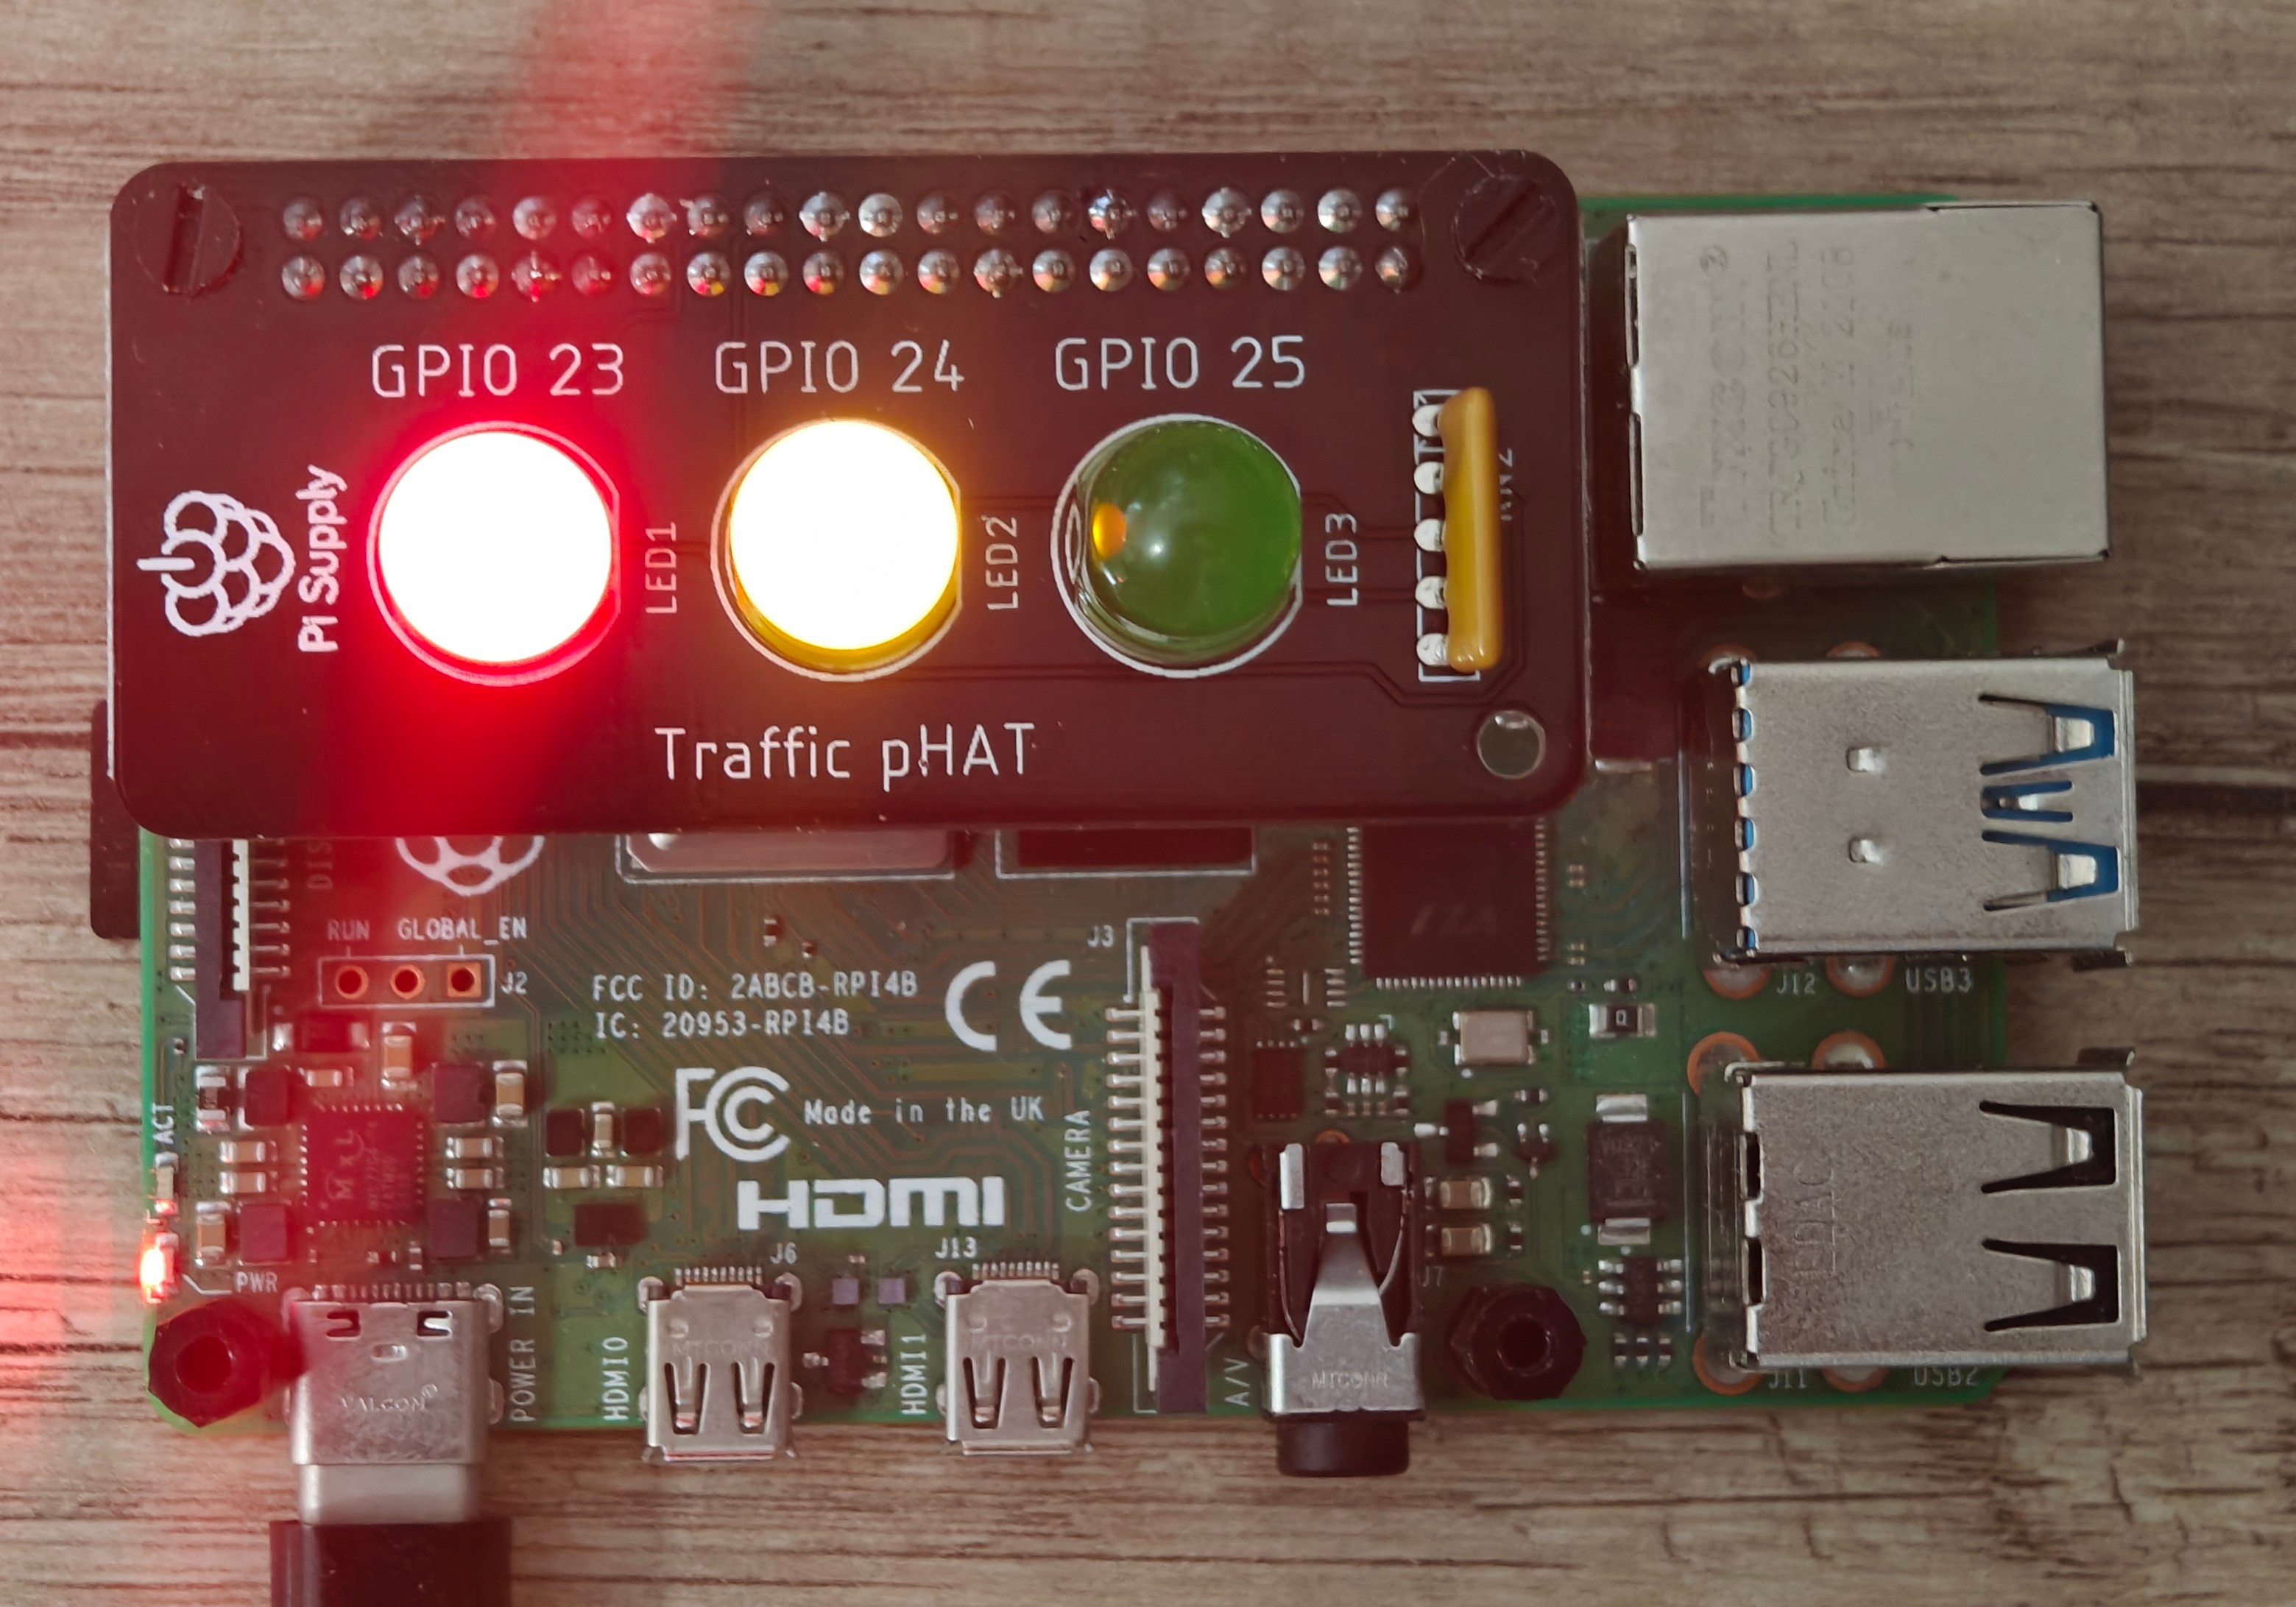
\includegraphics[width=0.6\linewidth]{media/traffic}
  \caption{Uruchomiony program piątego laboratorium}
  \label{fig:traffic}
\end{figure}
